\chapter{Results and discussion}
\label{Final results}

\section{Multi-disciplinary shape optimisation}
Two disciplines namely aerodynamics and structures which involves the calculation of aerodynamic drag ($ C_{DV} $) and von-mises ($ \sigma _{v} $) stress are considered for shape optimisation of airship profile. The aim is to have lowest possible aerodynamic drag and Von-Mises stress. To acieve this, we develop a composite objective function minimising which, both $ C_{DV} $ and $ \sigma _{v} $ are minimised simultaneously.
The objective function is defined as
\begin{equation}
F_{comp} = \frac{1}{2}\bigg( \frac{C_{DV}}{C_{DV,ref}} + \dfrac{\sigma _{v}}{\sigma _{v,ref}} \bigg)
\end{equation}

Where, $C_{DV,ref} , \sigma _{v,ref}  $ are the values of these parameters corresponding to the reference shape.  The values obtained in Table \ref{sub-optimal solution obtained} and \ref{Optimal solution obtained for mimimum sigma_v} are taken as reference values for $C_{DV,ref}$ and $\sigma _{v,ref}  $ respectively. The composite objective function now becomes:
\begin{equation}
\label{eqn f comp}
F_{comp} = 0.5*(55.67* C_{DV} + 2.607e-3 * \sigma _{v})
\end{equation}

Below table \ref{Optimal solution obtained for mimimum F comp} shows the optimal results obtained by minimising eqn. \ref{eqn f comp} using genetic algorithm. The obtained shape is shown in fig. \ref{Optimal F comp}. 

\begin{table}[H]
	\centering
	\caption{Optimal solution obtained for miminum $ F_{comp} $}
	\label{Optimal solution obtained for mimimum F comp}
	%\begin{ruledtabular}
	\begin{tabular}{lc}
		\hline \hline
		Design Parameters & Optimal value for minimum $ C_{DV} $    \\ \hline \hline
		
		$ Point\ of\ Max.\ Dia., m$ & 0.40942      \\  
		$ Nose\ Radius, r _{o} $ & 0.79999    \\
		$ Tail\ Radius, r _{1} $ & 0.30606    \\  
		$ Prismatic\ Coeff., C _{p }$ & 0.61508 \\
		$ Fineness\ Ratio, \frac{l}{d} $ & 5.75445 \\
		$Scaling\ in\ Y\ direction,\ scale\_y$ &1 \\ \hline \hline
		
		$ von-Mises\ stress\  \sigma _{v}  $ & 1.0253 \\
		\hline \hline
	\end{tabular}
	%	\end{ruledtabular}
\end{table}

\begin{figure}[H]
	\centering
	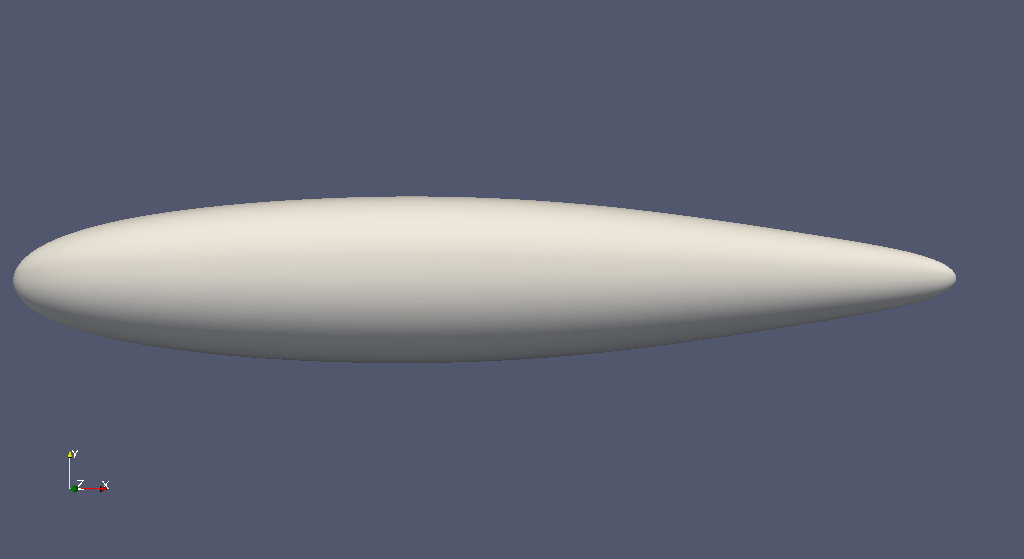
\includegraphics[width=300 pt]{rnd/min_f_comp.png}
	\caption{Optimal shape obtained for minimum composite objective function}
	\label{Optimal F comp} %      only if needed
\end{figure}
From table ref{Optimal solution obtained for mimimum F comp}, we can observe that the optimal shape for minimum $ F_{comp} $ is same as optimal shape for minimum $ c_{DV} $ shown in table \ref{optimal solution obtained}. This might be due to the fact that von-Mises stresses are not varying greatly with gertler parametres.